\documentclass{article}
\usepackage[utf8]{inputenc}
\usepackage[margin=2.5cm]{geometry}
\usepackage[version=4]{mhchem}
\usepackage{graphicx}
\usepackage{wrapfig}
\usepackage{placeins}
\usepackage{hyperref}
\usepackage{subcaption}

\setlength\parindent{0pt}

\begin{document}

\begin{titlepage}
    \begin{center}
        \vspace*{1cm}
        \Huge
        \textbf{Dr. Oetker food factory catastrophe! Chromatography}
        
        \vspace{0.5cm}
        \LARGE
        Chemistry 2 - TP 5
        
        \vspace{1.5cm}
        \textbf{Louis-Hendrik Barboutie}
        
        \vfill

        \includegraphics[width=0.4\textwidth]{logo_uni.jpg}
        
        \Large
        4$^{\underline{\text{th}}}$ May 2022
    \end{center}
\end{titlepage}

\section{Abstract}
The goal of this experiment was to separate via chromatography and identify with spectral analysis the compounds making up an unknown dye mixture. First a thin layer chromatography was performed to study the procedure, then the separation was performed using column chromatography. Finally, the spectral analysis allowed to identify brilliant blue and carmine as the unknown dyes.

\section{Introduction}
We are presented a dye mixture, a combination of two unknown dyes from lutein, curcumin, carmine or brilliant blue. The goal of this experiment session is to separate and identify these dyes with the liquid-solid chromatography method.

The method consists in having a solute being dragged along a solvent called mobile phase through a solid called stationary phase. If there is several compounds in the solute, they will be dragged along with differing rates, depending on the geometry of the molecule or their interactions with the mobile and stationary phases. The two types of chromatography we will use are thin layer chromatography (TLC) and column chromatography. In both of these silica will be the stationary phase. 

In TLC, the stationary phase consists of very tightly packed particles onto a plate. Due to adsorption, the solute and mobile phase will go up the TLC plate. The strength of the adsorption is linked to Vand der Waals attraction and dipole-dipole bonds, so changing the stationary phase to more polar molecules may increase the adsorption effect. Smaller particles will also reduce the ease of big molecules to traverse the TLC plate. 

In column chromatography gravity is used to pull the mobile phase and solute through the stationary phase. The overall process however is the same as for TLC, with the difference that it is possible to gather the separated compounds.

The four dyes at our disposition have various sizes and different solubilities, which can be exploited to separate them by chromatography. The topological representations of the dyes can be found in the appendix. The dyes are naturally coloured, and we can distinguish them by naked eye, but if this wasn't the case, and all the compounds were uncoloured, it would be necessary to perform spectral analysis. Lutein and curcumin are yellow pigments, while carmine is red and brilliant blue is, well, blue. In this way, it is possible to identify compounds with their spectrum.

Note that all the dyes are naturally occuring. Lutein and curcumin are organic, while carmine and brilliant blue can be obtained from minerals. 
\section{Experiment}

\subsection{Setup}

\subsubsection{Thin layer chromatography}

We have two TLC plates made of silica, which are the stationary phase. On both plates a very small amount of dye is deposited twice with the help of a capillary, such that the second deposit has double the amount of solute as for the first dot. Then, each plate is dipped into a different mobile phase: one in the brine solution and the other in the ethanol solution. The setup for the experiment is depicted in fig.~\ref{fig:setup1}.

\subsubsection{Column chromatography}

In this experiment, we change the stationary phase: in a column (a large burette) we put different layers (in order): some cotton wool, a small sand layer, a big silica gel layer, and finally a small sand layer again. Here the silica gel is the stationary phase. To perform the chromatography and the compound separation, the dye mixture is carefully deposited at the top of the column, and then solvent is continuously added. First we only use the brine solution for separating the red substance from the blue substance and then we use ethanol to flush the blue substance out of the column. A set of collection tubes is used to gather the solution coming out of the column. The used setup can be seen in fig.~\ref{fig:setup2}, where the chromatography is already ongoing.

For the identification of the substances, we will use a spectrophotometer in the UV-VIS range.

\begin{figure}[!ht]
    \centering
    \begin{subfigure}{0.49\textwidth}
        \centering
        \includegraphics[width=\textwidth]{Pictures/Setup1.jpg}
        \caption{TLC chromatography setup}
        \label{fig:setup1}
    \end{subfigure} 
    \begin{subfigure}{0.49\textwidth}
        \centering
        \includegraphics[width=\textwidth,angle=-90]{Pictures/Setup2.jpg}
        \caption{Column chromatography setup}
        \label{fig:setup2}
    \end{subfigure} 
\end{figure}
\FloatBarrier

\subsection{Employed chemicals}

\begin{enumerate}
    \item Dye mixture
    \item brine solution
    \item Ethanol
    \item Silica gel
\end{enumerate}

\subsection{Safety measures}
A lab coat, goggles and nitril gloves are mandatory to wear at all times for basic protection. Silica is irritating and has to be handled under a fumehood. Ethanol is highly flammable and is to be kept away from potential ignition sources.

\section{Results and discussion}

\subsection{Thin layer chromatography}

The final state of the TLC can be seen in fig.~\ref{fig:resultTLC}. A noticeable difference between the two TLCs is that the compounds do not travel in the same way in each. For a brine mobile phase, the two compounds do not move with the mobile phase front, whereas with the ethanol mobile phase they do. With ethanol, both compounds move at the same speed, but with brine, the blue compound barely leaves the beginning line. Additionally, the amount of a compound does not play a role in it's speed, the dot with twice the amount of mixture has the same retention as for the single dot. The two mobile phases also don't travel at the same speeds through the stationary phase, although that may be linked to the evaporation of ethanol, which might evaporate faster than it can reach the front.


\begin{figure}[!ht]
    \centering
    \includegraphics[width=0.5\textwidth,angle=-90]{Pictures/TLCanotated.jpg}
    \caption{Final state of the TLC chromatography}
    \label{fig:resultTLC}
\end{figure}
\FloatBarrier

A property of each compound, the retention factor, can be determined with the formula:

\begin{equation}
    \eta = \frac{d_{\text{solute}}}{d_{\text{mobile phase}}}
\end{equation}

Where $d_i$ is the distance travelled from the bottom line. It gives an indication as to how fast or how slow the solute moves with the mobile phase. With the values of the experiment, we obtain the following values for the retention factor:

\begin{table}[!ht]
    \centering
    \begin{tabular}{c|c|c}
         & ethanol & brine \\ \hline
        red compound & 1.00 & 0.74 \\
        blue compound & 1.00 & 0.10
    \end{tabular}
    \caption{Table of retention factors of the two compounds for both mobile phases}
    \label{tab:retentionFactor}
\end{table}

As seen in fig.~\ref{fig:resultTLC} and in tab.~\ref{tab:retentionFactor}, the red compound travels much faster in the brine mobile phase than the blue compound does. Both compounds travel at the same speed in an ethanol mobile phase. This knowledge can be used to separate them in a column chromatography: if we first use only brine solution as a mobile phase, both compounds will separate, and then we can finish the chromatography with the ethanol mobile phase, in which the blue compound travels faster.

\subsection{Column chromatography}
The column packing was not as successful as hoped, but still worked for the compound separation. When putting the layers on top of each other it was difficult to get a perfectly horizontal top line of the layer, especially for the silica gel. The sand could be shaken a bit into place, but this didn't work for the silica gel. Also the top layer of sand in the column was a bit too thin, which is why the compounds didn't separate in two distinct layers, but rather formed a gradient of colour.

Despite these difficulties, it was possible to separate the compounds, as seen in fig.~\ref{fig:testTubes}. Not all tubes contain only one compound though, since they weren't completely separated in the column, some dye mixture remained unseparated, which is why there are 2 tubes containing a purple solution. Two of the tubes, containing the most intense red and the most intense blue were then used for the spectrophotometry.  

\begin{figure}[!ht]
    \centering
    \includegraphics[width=0.8\textwidth]{Pictures/TestTubes1.jpg}
    \caption{Test tubes containing the separated compounds}
    \label{fig:testTubes}
\end{figure}

Luckily, our compounds can be differentiated by their colour, although this is not generally the case. We run a spectrophotometry nonetheless. The results are presented in fig.\ref{fig:absorbanceSpectrum}.

\begin{figure}[!ht]
    \centering
    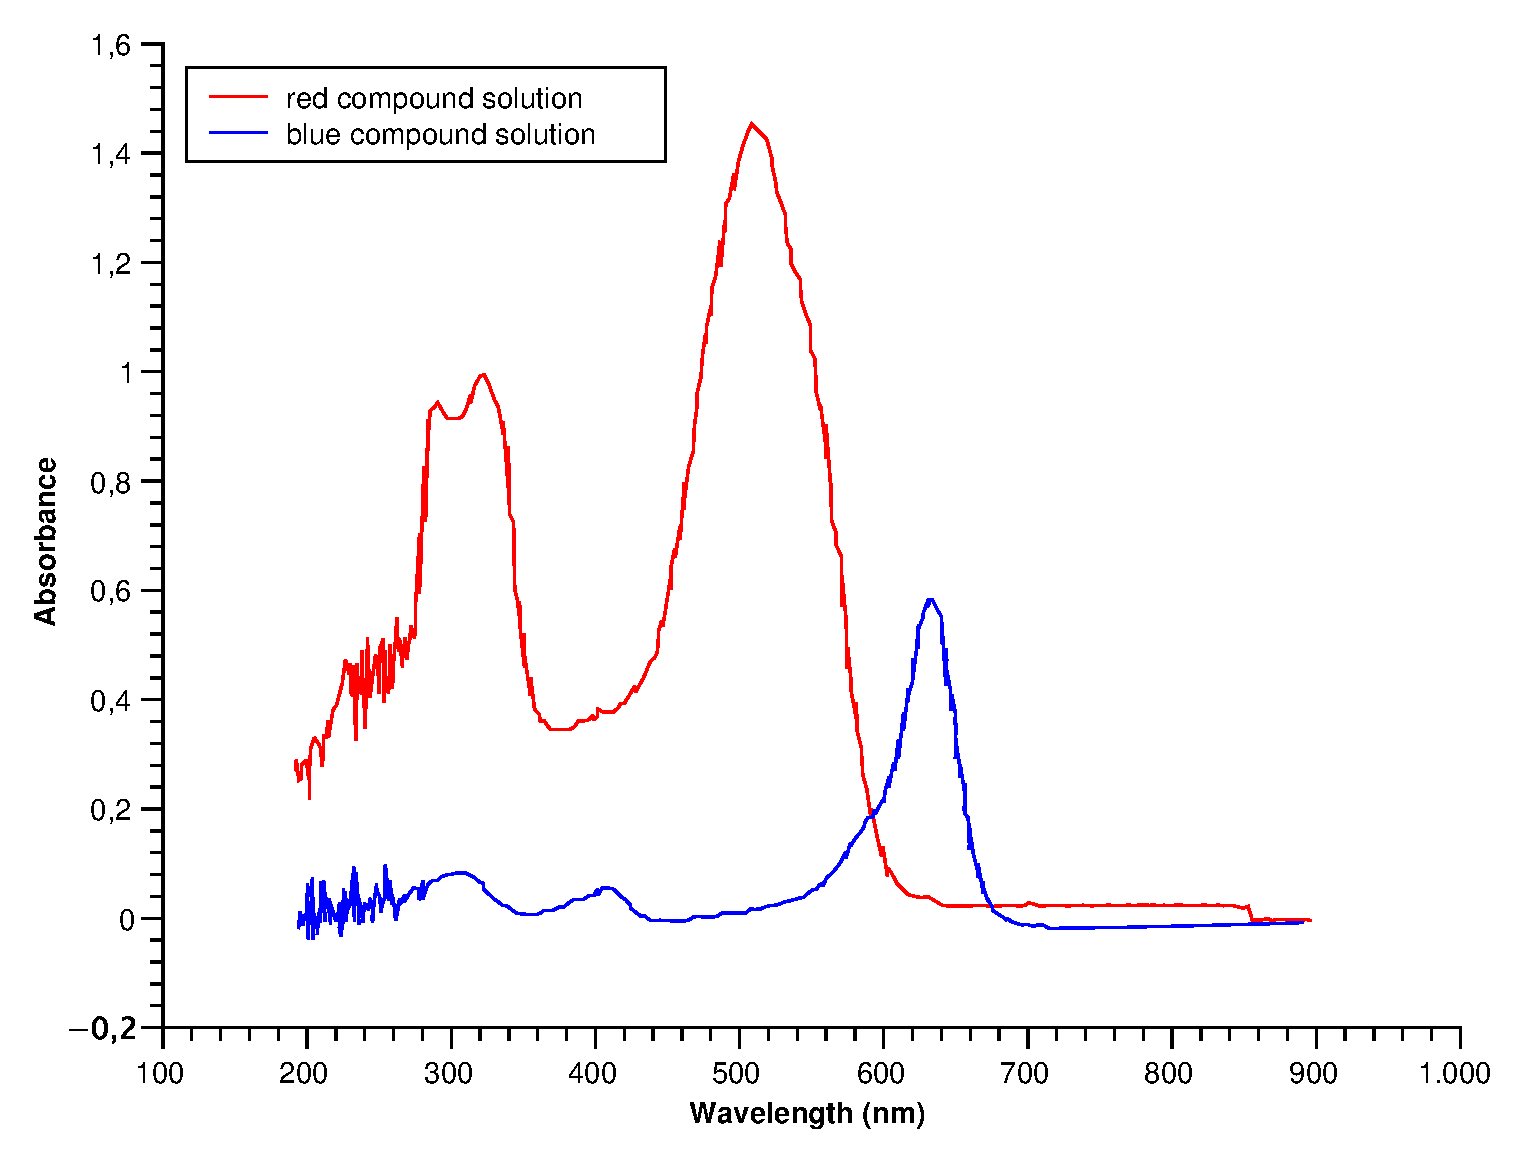
\includegraphics[width=0.5\textwidth]{Absorbance.eps}
    \caption{Absorbance of the red and blue solution in the UV-VIS range}
    \label{fig:absorbanceSpectrum}
\end{figure}
\FloatBarrier

As expected, the red solution has almost no absorbance for light of wavelength above 600 nm, and it absorbs blue light (500 nm) the most, but also UV light at ca. 320 nm. The blue solution absorbs red light the most in the range from 550-680 nm, and has absorbance peaks at 400 nm and 300 nm. This confirms what the colours that we see.
When comparing the absorbance spectra to the spectra of the proposed molecules, we can identify the blue compound to be brilliant blue, and the red compound to be carmine, both being non-toxic and safe for ingestion.

\section{Conclusion}

We have found that in TLC, the mobile phase plays an important role in the retention of the solute; the retention is however independent of the initial amount of solute. It has shown that it is possible to separate individual compounds from a mixture. We then succeeded in separating the two compounds and identified them to be carmine and brilliant blue.

The column chromatography could be improved in a few ways. We ran into the issue that there was no clear separation of the two dyes, but observed a gradient. A longer column, or different stationary phase and mobile phase pair could result in better separation (this excludes operator error). 

\vfill
\newpage

\section{Appendix}

\subsection{Lutein}

\begin{figure}[!ht]
    \centering
    \includegraphics[width=0.5\textwidth]{Molecules/Lutein_500.png}
    \caption{Lutein molecule}
    \label{fig:lutein}
\end{figure}
\FloatBarrier

\subsection{Curcumin}

\begin{figure}[!ht]
    \centering
    \includegraphics[width=0.5\textwidth]{Molecules/Curcumin_500.png}
    \caption{Curcumin molecule}
    \label{fig:curcumin}
\end{figure}
\FloatBarrier

\subsection{Carmine}

\begin{figure}[!ht]
    \centering
    \includegraphics[width=0.5\textwidth]{Molecules/Carmine_500.png}
    \caption{Carmine molecule}
    \label{fig:carmine}
\end{figure}
\FloatBarrier

\subsection{Brilliant blue}

\begin{figure}[!ht]
    \centering
    \includegraphics[width=0.5\textwidth]{Molecules/Brilliant_Blue_FCF_500.png}
    \caption{Brilliant blue molecule}
    \label{fig:brilliantBlue}
\end{figure}
\FloatBarrier

\subsection{Original absorbance spectra}

\begin{figure}
    \centering
    \includegraphics[width=\textwidth,angle=-90]{absorbanceog.jpg}
    \caption{Original absorbance spectra}
    \label{fig:OG_absorbi}
\end{figure}
\FloatBarrier

\begin{thebibliography}{}
    \bibitem{labguide} \textit{Dr. Oetker food factory catastrophe! Chromatography}, Lab guide, P. Dale, 2022
    \bibitem{lutein} \textit{Lutein}, PubChem, \url{https://pubchem.ncbi.nlm.nih.gov/compound/Lutein#section=2D-Structure}, last accessed 22/05/2022
    \bibitem{curcumin} \textit{Curcumin}, PubChem, \url{https://pubchem.ncbi.nlm.nih.gov/compound/curcumin#section=Structures}, last accessed 22/05/2022
    \bibitem{carmine} \textit{Carmine}, PubChem, \url{https://pubchem.ncbi.nlm.nih.gov/compound/Carmine#section=Structures}, last accessed 22/05/2022
    \bibitem{brilliantBlue} \textit{Brilliant Blue FCF}, PubChem, \url{https://pubchem.ncbi.nlm.nih.gov/compound/Brilliant-Blue-FCF}, last accessed 22/05/2022
\end{thebibliography}

\end{document}
